\documentclass[addpoints, 12pt]{exam}

\usepackage{amsmath}
\usepackage{tikz}
%\usepackage[latin1]{inputenc}
\usetikzlibrary{shapes,arrows}
\usetikzlibrary{calc,arrows,through}
\usetikzlibrary{intersections}
\usepackage{multicol}
\usepackage{yhmath}
\usepackage{lscape}

\pagestyle{empty}

\tikzstyle{line} = [draw, -triangle 45]

\newcommand{\linedraw}[2]{
	\draw [line] (#2)--($(#2)!.5cm!180:(#1)$);
	\draw [line] (#2)--($(#1)!.5cm!180:(#2)$);
}

\newcommand{\raydraw}[2]{
	\draw [line] (#1)--($(#2)!.5cm!180:(#1)$);
}

\newcommand{\fillpoints}[1]{
	\foreach \point in {#1} \fill (\point) circle (2.5pt);
}

\begin{document}

\begin{tabbing}
\noindent Name: \rule[-0.1cm]{5cm}{0.01cm} \hspace{2.5in}  \\
Precalculus*: Graphing Trigonometric Functions (Radians)  
\end{tabbing}

\vspace{1cm}

\begin{center}
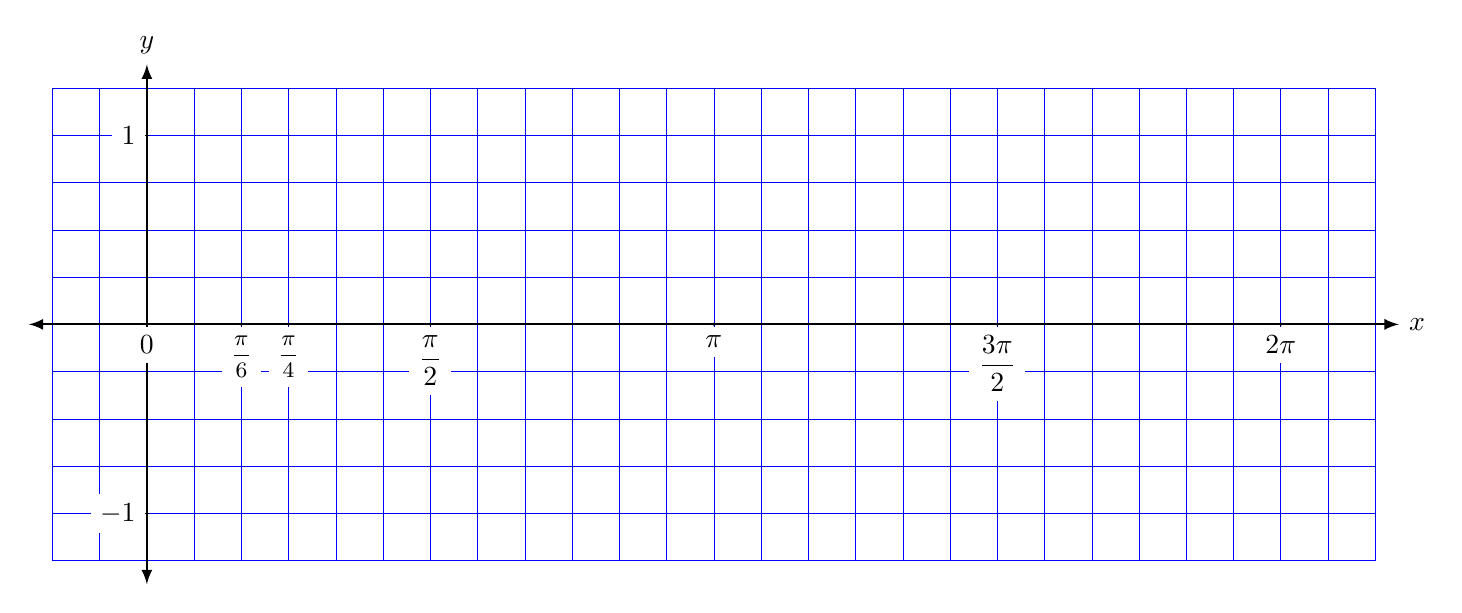
\begin{tikzpicture} [scale=0.6]

		\draw [help lines,blue] (-2,-5) grid (26,5);
		\draw [thick,latex-latex] (-2.5,0)--(26.5,0) node [right] {$x$};
		\draw [thick,latex-latex] (0,-5.5)--(0,5.5) node [above] {$y$};	

		\foreach \x in {0} 
			\draw (\x cm,1pt) -- (\x,-1pt)	node[anchor=north,fill=white]{$0$};
		\foreach \x in {2} 
			\draw (\x cm,1pt) -- (\x,-1pt)	node[anchor=north,fill=white]{\footnotesize $\dfrac{\pi}{6}$};
		\foreach \x in {3} 
			\draw (\x cm,1pt) -- (\x,-1pt)	node[anchor=north,fill=white]{\footnotesize $\dfrac{\pi}{4}$};	
		\foreach \x in {6} 
			\draw (\x cm,1pt) -- (\x,-1pt)	node[anchor=north,fill=white]{$\dfrac{\pi}{2}$};
		\foreach \x in {12} 
			\draw (\x cm,1pt) -- (\x,-1pt)	node[anchor=north,fill=white]{$\pi$};
		\foreach \x in {18} 
			\draw (\x cm,1pt) -- (\x,-1pt)	node[anchor=north,fill=white]{$\dfrac{3\pi}{2}$};
		\foreach \x in {24} 
			\draw (\x cm,1pt) -- (\x,-1pt)	node[anchor=north,fill=white]{$2\pi$};			
		\foreach \y in {4} 
			\draw (1pt, \y cm) -- (-1 pt, \y cm) node[anchor=east,fill=white] {$1$};
		\foreach \y in {-4} 
			\draw (1pt, \y cm) -- (-1 pt, \y cm) node[anchor=east,fill=white] {$-1$};	
	
\end{tikzpicture}
\end{center}

\vspace{2cm}


\begin{center}
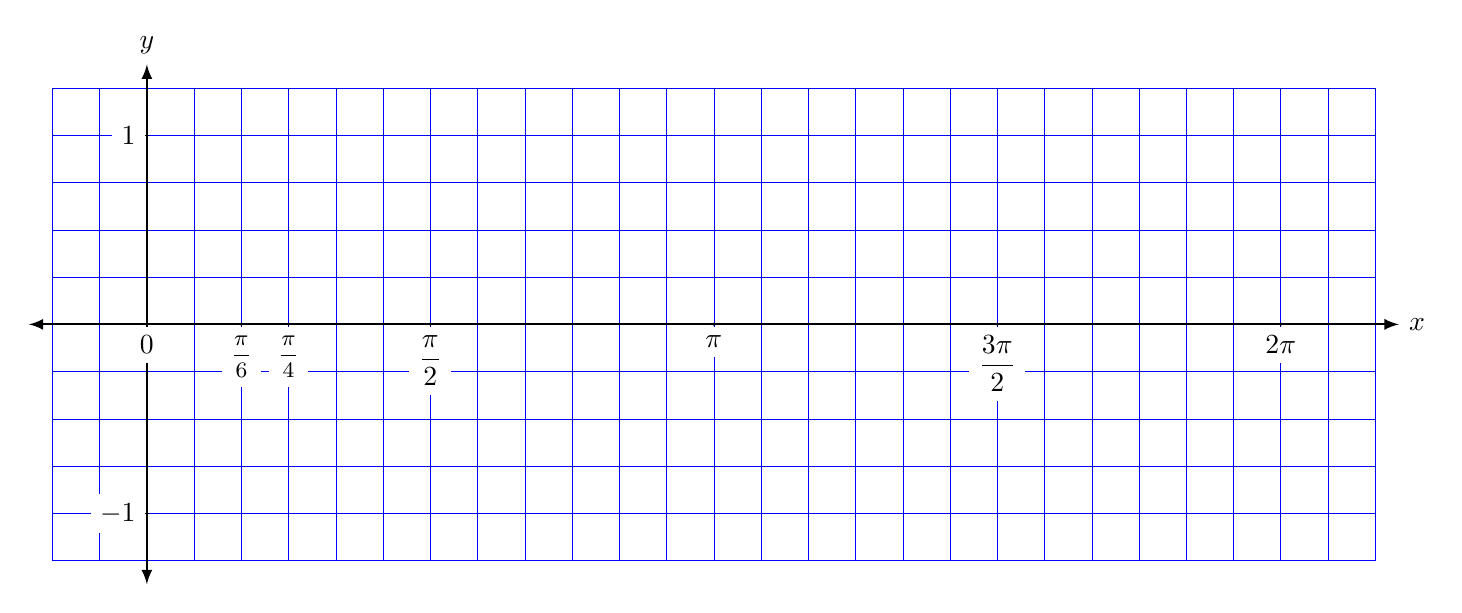
\begin{tikzpicture} [scale=0.6]

		\draw [help lines,blue] (-2,-5) grid (26,5);
		\draw [thick,latex-latex] (-2.5,0)--(26.5,0) node [right] {$x$};
		\draw [thick,latex-latex] (0,-5.5)--(0,5.5) node [above] {$y$};	

		\foreach \x in {0} 
			\draw (\x cm,1pt) -- (\x,-1pt)	node[anchor=north,fill=white]{$0$};
		\foreach \x in {2} 
			\draw (\x cm,1pt) -- (\x,-1pt)	node[anchor=north,fill=white]{\footnotesize $\dfrac{\pi}{6}$};
		\foreach \x in {3} 
			\draw (\x cm,1pt) -- (\x,-1pt)	node[anchor=north,fill=white]{\footnotesize $\dfrac{\pi}{4}$};	
		\foreach \x in {6} 
			\draw (\x cm,1pt) -- (\x,-1pt)	node[anchor=north,fill=white]{$\dfrac{\pi}{2}$};
		\foreach \x in {12} 
			\draw (\x cm,1pt) -- (\x,-1pt)	node[anchor=north,fill=white]{$\pi$};
		\foreach \x in {18} 
			\draw (\x cm,1pt) -- (\x,-1pt)	node[anchor=north,fill=white]{$\dfrac{3\pi}{2}$};
		\foreach \x in {24} 
			\draw (\x cm,1pt) -- (\x,-1pt)	node[anchor=north,fill=white]{$2\pi$};			
		\foreach \y in {4} 
			\draw (1pt, \y cm) -- (-1 pt, \y cm) node[anchor=east,fill=white] {$1$};
		\foreach \y in {-4} 
			\draw (1pt, \y cm) -- (-1 pt, \y cm) node[anchor=east,fill=white] {$-1$};	
	
\end{tikzpicture}
\end{center}

\newpage

\begin{landscape}


\begin{flushleft}
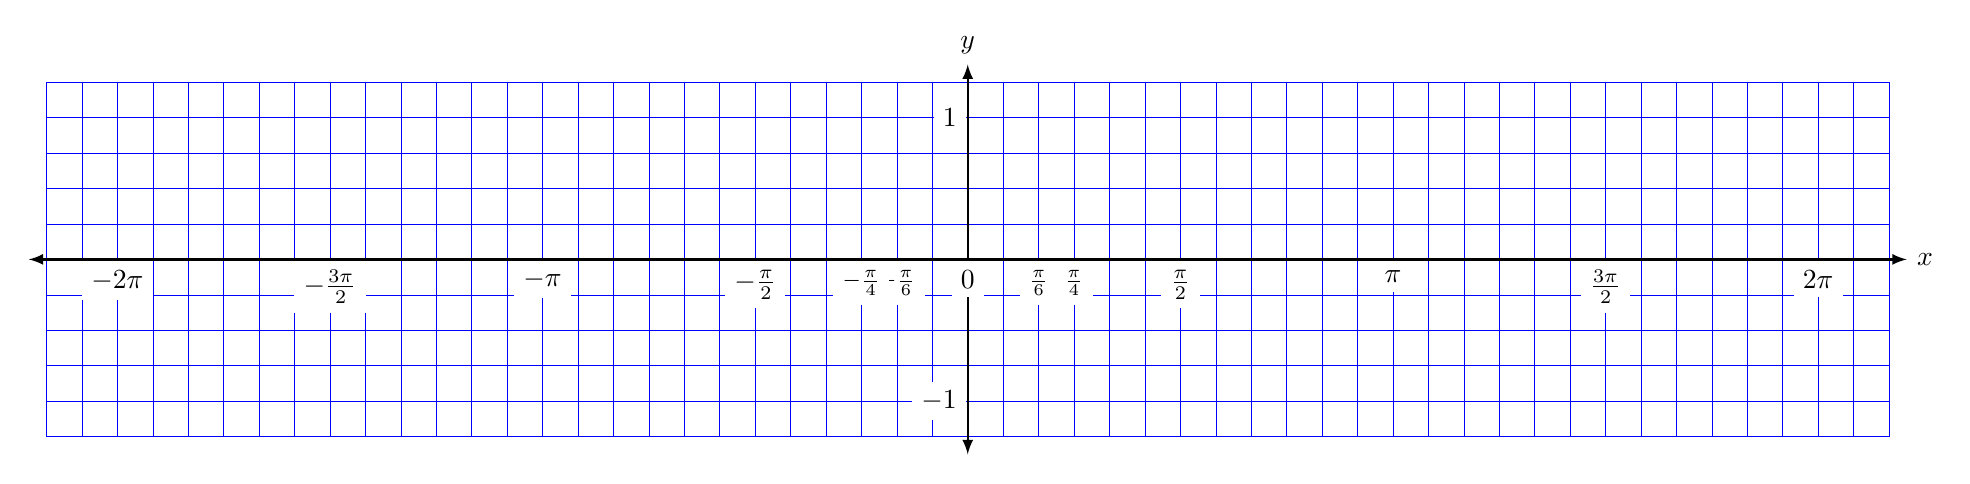
\begin{tikzpicture} [scale=0.45]

		\draw [help lines,blue] (-26,-5) grid (26,5);
		\draw [thick,latex-latex] (-26.5,0)--(26.5,0) node [right] {$x$};
		\draw [thick,latex-latex] (0,-5.5)--(0,5.5) node [above] {$y$};	

		\foreach \x in {0} 
			\draw (\x cm,1pt) -- (\x,-1pt)	node[anchor=north,fill=white]{$0$};
		\foreach \x in {2} 
			\draw (\x cm,1pt) -- (\x,-1pt)	node[anchor=north,fill=white]{\footnotesize $\frac{\pi}{6}$};
		\foreach \x in {-2} 	
			\draw (\x cm,1pt) -- (\x,-1pt)	node[anchor=north,fill=white]{\footnotesize $-\frac{\pi}{6}$};
		\foreach \x in {3} 
			\draw (\x cm,1pt) -- (\x,-1pt)	node[anchor=north,fill=white]{\footnotesize $\frac{\pi}{4}$};	
		\foreach \x in {-3} 
			\draw (\x cm,1pt) -- (\x,-1pt)	node[anchor=north,fill=white]{\footnotesize $-\frac{\pi}{4}$};	
		\foreach \x in {6} 
			\draw (\x cm,1pt) -- (\x,-1pt)	node[anchor=north,fill=white]{$\frac{\pi}{2}$};
		\foreach \x in {-6} 
			\draw (\x cm,1pt) -- (\x,-1pt)	node[anchor=north,fill=white]{$-\frac{\pi}{2}$};	
		\foreach \x in {12} 
			\draw (\x cm,1pt) -- (\x,-1pt)	node[anchor=north,fill=white]{$\pi$};
			\foreach \x in {-12} 
			\draw (\x cm,1pt) -- (\x,-1pt)	node[anchor=north,fill=white]{$-\pi$};
		\foreach \x in {18} 
			\draw (\x cm,1pt) -- (\x,-1pt)	node[anchor=north,fill=white]{$\frac{3\pi}{2}$};
		\foreach \x in {-18} 
			\draw (\x cm,1pt) -- (\x,-1pt)	node[anchor=north,fill=white]{$-\frac{3\pi}{2}$};	
		\foreach \x in {24} 
			\draw (\x cm,1pt) -- (\x,-1pt)	node[anchor=north,fill=white]{$2\pi$};
		\foreach \x in {-24} 
			\draw (\x cm,1pt) -- (\x,-1pt)	node[anchor=north,fill=white]{$-2\pi$};				
		\foreach \y in {4} 
			\draw (1pt, \y cm) -- (-1 pt, \y cm) node[anchor=east,fill=white] {$1$};
		\foreach \y in {-4} 
			\draw (1pt, \y cm) -- (-1 pt, \y cm) node[anchor=east,fill=white] {$-1$};	
	
\end{tikzpicture}
\end{flushleft}


\vspace{2cm}

\begin{flushleft}
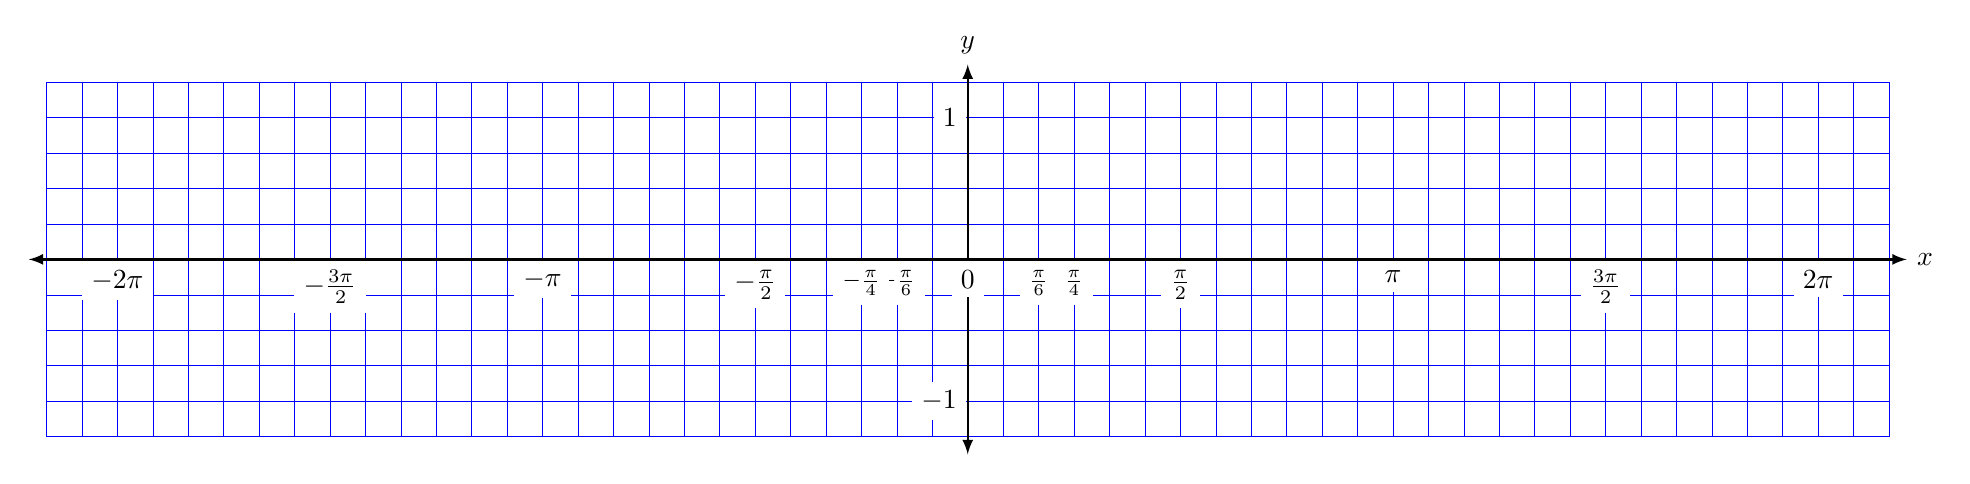
\begin{tikzpicture} [scale=0.45]

		\draw [help lines,blue] (-26,-5) grid (26,5);
		\draw [thick,latex-latex] (-26.5,0)--(26.5,0) node [right] {$x$};
		\draw [thick,latex-latex] (0,-5.5)--(0,5.5) node [above] {$y$};	

		\foreach \x in {0} 
			\draw (\x cm,1pt) -- (\x,-1pt)	node[anchor=north,fill=white]{$0$};
		\foreach \x in {2} 
			\draw (\x cm,1pt) -- (\x,-1pt)	node[anchor=north,fill=white]{\footnotesize $\frac{\pi}{6}$};
		\foreach \x in {-2} 	
			\draw (\x cm,1pt) -- (\x,-1pt)	node[anchor=north,fill=white]{\footnotesize $-\frac{\pi}{6}$};
		\foreach \x in {3} 
			\draw (\x cm,1pt) -- (\x,-1pt)	node[anchor=north,fill=white]{\footnotesize $\frac{\pi}{4}$};	
		\foreach \x in {-3} 
			\draw (\x cm,1pt) -- (\x,-1pt)	node[anchor=north,fill=white]{\footnotesize $-\frac{\pi}{4}$};	
		\foreach \x in {6} 
			\draw (\x cm,1pt) -- (\x,-1pt)	node[anchor=north,fill=white]{$\frac{\pi}{2}$};
		\foreach \x in {-6} 
			\draw (\x cm,1pt) -- (\x,-1pt)	node[anchor=north,fill=white]{$-\frac{\pi}{2}$};	
		\foreach \x in {12} 
			\draw (\x cm,1pt) -- (\x,-1pt)	node[anchor=north,fill=white]{$\pi$};
			\foreach \x in {-12} 
			\draw (\x cm,1pt) -- (\x,-1pt)	node[anchor=north,fill=white]{$-\pi$};
		\foreach \x in {18} 
			\draw (\x cm,1pt) -- (\x,-1pt)	node[anchor=north,fill=white]{$\frac{3\pi}{2}$};
		\foreach \x in {-18} 
			\draw (\x cm,1pt) -- (\x,-1pt)	node[anchor=north,fill=white]{$-\frac{3\pi}{2}$};	
		\foreach \x in {24} 
			\draw (\x cm,1pt) -- (\x,-1pt)	node[anchor=north,fill=white]{$2\pi$};
		\foreach \x in {-24} 
			\draw (\x cm,1pt) -- (\x,-1pt)	node[anchor=north,fill=white]{$-2\pi$};				
		\foreach \y in {4} 
			\draw (1pt, \y cm) -- (-1 pt, \y cm) node[anchor=east,fill=white] {$1$};
		\foreach \y in {-4} 
			\draw (1pt, \y cm) -- (-1 pt, \y cm) node[anchor=east,fill=white] {$-1$};	
	
\end{tikzpicture}
\end{flushleft}


\vspace{2cm}

\end{landscape}

\end{document}